\documentclass[a4paper,12pt]{article}

\usepackage{graphicx}
\usepackage{hyperref}
\usepackage{caption,subcaption}
\usepackage{xcolor}
\usepackage{ctex}
\usepackage{geometry}
\usepackage{tikz}
\usepackage{comment}
\usepackage{xifthen}
\usepackage{titlesec}
\usepackage{forloop}
\usepackage{lastpage}
\usepackage{totcount}
\usepackage[inline, shortlabels]{enumitem}
\usepackage{amsmath}
\usepackage{array}

% section counter
\newtotcounter{section_cnt}

% set page
\geometry{left=2cm,right=2cm,top=3cm,bottom=2cm}

% section format
\renewcommand\thesection{\Alph{section}}
\titleformat{\section}[block]{\Huge\filcenter\textbf}{\thesection.}{1em}{}
\titleformat{\subsection}[hang]{\bfseries}{}{1em}{}

% count section
\usepackage{letltxmacro}
\LetLtxMacro{\oldsection}{\section} \renewcommand{\section}[1]{\oldsection{#1}\label{\thesection}\stepcounter{section_cnt}}

% input tex files
\renewcommand{\include}[1]{\input{"#1.tex"}}

% set enumerate padding
\setenumerate[1]{itemsep=0pt,partopsep=0pt,parsep=\parskip,topsep=0pt}
\setitemize[1]{itemsep=0pt,partopsep=0pt,parsep=\parskip,topsep=0pt}

\usepackage{xargs}

\newcommandx{\MakeLimits}[2][1=1000 ms, 2=65536 kB]{
    \begin{center}
        \large{Time Limit: #1 \hspace{20pt} Memory Limit: #2}
    \end{center}
}

\title{\textbf{PKU Campus 2019\\Contest Problem Set}}
\date{\textbf{May 12th, 2019}}
\author{\textbf{Peking University}}

\begin{document}
\maketitle

\label{FirstPage}

\vspace{90pt}
\begin{center}
This problem set contains \number\totvalue{section_cnt} problems; pages are numbered from \pageref{FirstPage} to \pageref{LastPage}.
\end{center}

\vspace{90pt}
\textbf{Attention:}
\begin{enumerate}
    \item The input must be read from standard input.
    \item The output must be written to standard output.
    \item If you use long long in your gcc/g++ program, make sure you use ``\%lld'' instead of ``\%I64d'' while reading or writing long long value.
    \item Due to possible changes during the contest, please refresh the web frequently.
\end{enumerate}

\clearpage{}

\newgeometry{left=2cm,right=2cm,top=4.8cm,bottom=2cm}

\newcommand{\addline}[1]{\rule{0pt}{2.1em} \Large{\ref{#1}} & 
\Large{\nameref{#1}} & \Large{\pageref{#1}} \\ [1ex] }

\begin{table}[ht]

\centering
\caption*{\Huge{Problem List}}

\newcounter{it}
\begin{tabular}{>{\centering\arraybackslash}p{1.8cm} c >{\centering\arraybackslash}p{1.8cm}}
\hline
\rule{0pt}{2.4em} \LARGE{ID} & \LARGE{Title} & \LARGE{Page} \\ [1ex]
\hline
  \setcounter{it}{1}
  \whiledo{\theit<\totvalue{section_cnt}}{
    \addline{\Alph{it}}
    \stepcounter{it}
  }
  \addline{\Alph{it}}
  \hline
\end{tabular}

\end{table}
\restoregeometry
\clearpage{}

\section{Wu Xing}

\MakeLimits[1000 ms][65536 kB]

\subsection{Description}

The Wu Xing, or the Five Elements, is very much a part of Chinese traditional culture. It plays an important part in ancient Chinese geomancy, astrology, medicine, music, military strategy, martial arts, etc.

The Wu Xing is comprised of five elements: earth, fire, metal, water and wood. There is either a generating or an overcoming interaction between each pair of different elements. These two kinds of interactions are illustrated by the picture below:

\begin{center}
    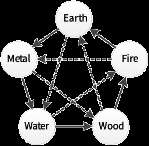
\includegraphics[]{pics/wuxing.jpeg}
\end{center}

A solid arrow from A to B means "A generates B", and a dotted arrow from A to B means "A overcomes B".

Now give you some pairs of different elements, please figure out the interaction between each pair.

\subsection{Input Format}

The first line contains an integer $N$, indicates the number of pairs of different elements.

Then $N$ lines follow. Each line contains a pair of strings $S_1$ and $S_2$, separated by a single space. Both $S_1$ and $S_2$ are one of the following five strings: "earth", "fire", "metal", "water", or "wood". $S_1$ and $S_2$ are different and indicate a pair of elements.

\subsection{Output Format}

For each pair of different elements $S_1$ and $S_2$, output a sentence in a single line in one of the four formats below, according to the interaction between them:
$S_1$ generates $S_2$.
$S_2$ generates $S_1$.
$S_1$ overcomes $S_2$.
$S_2$ overcomes $S_1$.

Note that for each sentence, there is a period (".") at the end and the first letter should be capitalized.

\subsection{Sample Input}
\begin{data}
2

earth water

earth fire
\end{data}
\subsection{Sample Output}
\begin{data}
Earth overcomes water.

Fire generates earth.
\end{data}

\clearpage{}

\section{Template}

\subsection{Description}

\subsection{Input Format}

\subsection{Output Format}

\subsection{Sample Input}

\subsection{Sample Output}

\clearpage{}

\end{document}

